\chapter{Le 5 octobre}

\lettrine{I}{l} était six heures du soir à peu près, un jour couleur d'opale, dans lequel un beau soleil d'automne infiltrait ses rayons d'or, tombait du ciel sur la mer bleuâtre. 

\zz
La chaleur du jour s'était éteinte graduellement, et l'on commençait à sentir cette légère brise qui semble la respiration de la nature se réveillant après la sieste brûlante du midi, souffle délicieux qui rafraîchit les côtes de la Méditerranée et qui porte de rivage en rivage le parfum des arbres, mêlé à l'âcre senteur de la mer. 

Sur cet immense lac qui s'étend de Gibraltar aux Dardanelles et de Tunis à Venise, un léger yacht, pur et élégant de forme, glissait dans les premières vapeurs du soir. Son mouvement était celui du cygne qui ouvre ses ailes au vent et qui semble glisser sur l'eau. Il s'avançait, rapide et gracieux à la fois, et laissant derrière lui un sillon phosphorescent. 

Peu à peu le soleil, dont nous avons salué les derniers rayons, avait disparu à l'horizon occidental; mais, comme pour donner raison aux rêves brillants de la mythologie, ses feux indiscrets, reparaissant au sommet de chaque vague, semblaient révéler que le dieu de flamme venait de se cacher au sein d'Amphitrite, qui essayait en vain de cacher son amant dans les plis de son manteau azuré. 

Le yacht avançait rapidement, quoique en apparence il y eût à peine assez de vent pour faire flotter la chevelure bouclée d'une jeune fille. 

Debout sur la proue, un homme de haute taille, au teint de bronze, à l'œil dilaté, voyait venir à lui la terre sous la forme d'une masse sombre disposée en cône, et sortant du milieu des flots comme un immense chapeau de Catalan. 

«Est-ce là Monte-Cristo? demanda d'une voix grave et empreinte d'une profonde tristesse le voyageur aux ordres duquel le petit yacht semblait être momentanément soumis. 

—Oui, Excellence, répondit le patron, nous arrivons. 

—Nous arrivons!» murmura le voyageur avec un indéfinissable accent de mélancolie. 

Puis il ajouta à voix basse: 

«Oui, ce sera là le port.» 

Et il se replongea dans sa pensée, qui se traduisait par un sourire plus triste que ne l'eussent été des larmes. 

Quelques minutes après, on aperçut à terre la lueur d'une flamme qui s'éteignit aussitôt, et le bruit d'une arme à feu arriva jusqu'au yacht. 

«Excellence, dit le patron, voici le signal de terre, voulez-vous y répondre vous-même? 

—Quel signal?» demanda celui-ci. 

Le patron étendit la main vers l'île aux flancs de laquelle montait, isolé et blanchâtre, un large flocon de fumée qui se déchirait en s'élargissant. 

«Ah! oui, dit-il, comme sortant d'un rêve, donnez.» 

Le patron lui tendit une carabine toute chargée, le voyageur la prit, la leva lentement et fit feu en l'air. 

Dix minutes après on carguait les voiles, et l'on jetait l'ancre à cinq cents pas d'un petit port. 

Le canot était déjà à la mer avec quatre rameurs et le pilote; le voyageur descendit, et au lieu de s'asseoir à la poupe, garnie pour lui d'un tapis bleu, se tint debout et les bras croisés. 

Les rameurs attendaient, leurs avirons à demi levés, comme des oiseaux qui font sécher leurs ailes. 

«Allez!» dit le voyageur. 

Les huit rames retombèrent à la mer d'un seul coup et sans faire jaillir une goutte d'eau; puis la barque, cédant à l'impulsion, glissa rapidement. 

En un instant on fut dans une petite anse formée par une échancrure naturelle, la barque toucha sur un fond de sable fin. 

«Excellence, dit le pilote, montez sur les épaules de deux de nos hommes, ils vous porteront à terre.» 

Le jeune homme répondit à cette invitation par un geste de complète indifférence, dégagea ses jambes de la barque et se laissa glisser dans l'eau qui lui monta jusqu'à la ceinture. 

«Ah! Excellence, murmura le pilote, c'est mal ce que vous faites là, et vous nous ferez gronder par le maître.» 

Le jeune homme continua d'avancer vers le rivage, suivant deux matelots qui choisissaient le meilleur fond. 

Au bout d'une trentaine de pas on avait abordé; le jeune homme secouait ses pieds sur un terrain sec, et cherchait des yeux autour de lui le chemin probable qu'on allait lui indiquer, car il faisait tout à fait nuit. 

Au moment où il tournait la tête, une main se posait sur son épaule, et une voix le fit tressaillir. 

«Bonjour, Maximilien, disait cette voix, vous êtes exact, merci! 

—C'est vous, comte, s'écria le jeune homme avec un mouvement qui ressemblait à de la joie, et en serrant de ses deux mains la main de Monte-Cristo. 

—Oui, vous le voyez, aussi exact que vous; mais vous êtes ruisselant, mon cher ami: il faut vous changer, comme dirait Calypso à Télémaque. Venez donc, il y a par ici une habitation toute préparée pour vous, dans laquelle vous oublierez fatigues et froid.» 

Monte-Cristo s'aperçut que Morrel se retournait; il attendit. 

Le jeune homme, en effet, voyait avec surprise que pas un mot n'avait été prononcé par ceux qui l'avaient amené, qu'il ne les avait pas payés et que cependant ils étaient partis. On entendait même déjà le battement des avirons de la barque qui retournait vers le petit yacht. 

«Ah! oui, dit le comte, vous cherchez vos matelots? 

—Sans doute, je ne leur ai rien donné, et cependant ils sont partis. 

—Ne vous occupez point de cela, Maximilien, dit en riant Monte-Cristo, j'ai un marché avec la marine pour que l'accès de mon île soit franc de tout droit de charroi et de voyage. Je suis abonné, comme on dit dans les pays civilisés.» 

Morrel regarda le comte avec étonnement. 

«Comte, lui dit-il, vous n'êtes plus le même qu'à Paris. 

—Comment cela? 

—Oui, ici, vous riez.» 

Le front de Monte-Cristo s'assombrit tout à coup. 

«Vous avez raison de me rappeler à moi-même, Maximilien, dit-il, vous revoir était un bonheur pour moi, et j'oubliais que tout bonheur est passager. 

—Oh! non, non, comte! s'écria Morrel en saisissant de nouveau les deux mains de son ami; riez au contraire, soyez heureux, vous, et prouvez-moi par votre indifférence que la vie n'est mauvaise qu'à ceux qui souffrent. Oh! vous êtes charitable; vous êtes bon, vous êtes grand, mon ami, et c'est pour me donner du courage que vous affectez cette gaieté. 

—Vous vous trompez, Morrel, dit Monte-Cristo, c'est qu'en effet j'étais heureux. 

—Alors vous m'oubliez moi-même; tant mieux! 

—Comment cela? 

—Oui, car vous le savez, ami, comme disait le gladiateur entrant dans le cirque au sublime empereur, je vous dis à vous: «Celui qui va mourir te salue.» 

—Vous n'êtes pas consolé? demanda Monte-Cristo avec un regard étrange. 

—Oh! fit Morrel avec un regard plein d'amertume, avez-vous cru réellement que je pouvais l'être? 

—Écoutez, dit le comte, vous entendez bien mes paroles, n'est-ce pas, Maximilien? Vous ne me prenez pas pour un homme vulgaire, pour une crécelle qui émet des sons vagues et vides de sens. Quand je vous demande si vous êtes consolé, je vous parle en homme pour qui le cœur humain n'a plus de secret. Eh bien, Morrel, descendons ensemble au fond de votre cœur et sondons-le. Est-ce encore cette impatience fougueuse de douleur qui fait bondir le corps comme bondit le lion piqué par le moustique? Est-ce toujours cette soif dévorante qui ne s'éteint que dans la tombe? Est-ce cette idéalité du regret qui lance le vivant hors de la vie à la poursuite du mort? ou bien est-ce seulement la prostration du courage épuisé, l'ennui qui étouffe le rayon d'espoir qui voudrait luire? est-ce la perte de la mémoire, amenant l'impuissance des larmes? Oh! mon cher ami, si c'est cela, si vous ne pouvez plus pleurer, si vous croyez mort votre cœur engourdi, si vous n'avez plus de force qu'en Dieu, de regards que pour le ciel, ami, laissons de côté les mots trop étroits pour le sens que leur donne notre âme. Maximilien, vous êtes consolé, ne vous plaignez plus. 

—Comte, dit Morrel de sa voix douce et ferme en même temps; comte, écoutez-moi, comme on écoute un homme qui parle le doigt étendu vers la terre, les yeux levés au ciel: je suis venu près de vous pour mourir dans les bras d'un ami. Certes, il est des gens que j'aime: j'aime ma sœur Julie, j'aime son mari Emmanuel; mais j'ai besoin qu'on m'ouvre des bras forts et qu'on me sourie à mes derniers instants; ma sœur fondrait en larmes et s'évanouirait; je la verrais souffrir, et j'ai assez souffert; Emmanuel m'arracherait l'arme des mains et remplirait la maison de ses cris. Vous, comte, dont j'ai la parole, vous qui êtes plus qu'un homme, vous que j'appellerais un dieu si vous n'étiez mortel, vous, vous me conduirez doucement et avec tendresse, n'est-ce pas, jusqu'aux portes de la mort? 

—Ami, dit le comte, il me reste encore un doute: auriez-vous si peu de force, que vous mettiez de l'orgueil à étaler votre douleur? 

—Non, voyez, je suis simple, dit Morrel en tendant la main au comte, et mon pouls ne bat ni plus fort ni plus lentement que d'habitude. Non, je me sens au bout de la route; non, je n'irai pas plus loin. Vous m'avez parlé d'attendre et d'espérer; savez-vous ce que vous avez fait, malheureux sage que vous êtes? J'ai attendu un mois, c'est-à-dire que j'ai souffert un mois! J'ai espéré (l'homme est une pauvre et misérable créature), j'ai espéré, quoi? je n'en sais rien, quelque chose d'inconnu, d'absurde, d'insensé! un miracle\dots lequel? Dieu seul peut le dire, lui qui a mêlé à notre raison cette folie que l'on nomme espérance. Oui, j'ai attendu; oui, j'ai espéré, comte, et depuis un quart d'heure que nous parlons vous m'avez cent fois, sans le savoir, brisé, torturé le cœur, car chacune de vos paroles m'a prouvé qu'il n'y a plus d'espoir pour moi. Ô comte! que je reposerai doucement et voluptueusement dans la mort!» 

Morrel prononça ces derniers mots avec une explosion d'énergie qui fit tressaillir le comte. 

«Mon ami, continua Morrel, voyant que le comte se taisait, vous m'avez désigné le 5 octobre comme le terme du sursis que vous me demandiez\dots mon ami, c'est aujourd'hui le 5 octobre\dots» 

Morrel tira sa montre. 

«Il est neuf heures, j'ai encore trois heures à vivre. 

—Soit, répondit Monte-Cristo, venez.» 

Morrel suivit machinalement le comte, et ils étaient déjà dans la grotte que Maximilien ne s'en était pas encore aperçu. 

Il trouva des tapis sous ses pieds, une porte s'ouvrit, des parfums l'enveloppèrent, une vive lumière frappa ses yeux. 

Morrel s'arrêta, hésitant à avancer; il se défiait des énervantes délices qui l'entouraient. 

Monte-Cristo l'attira doucement. 

«Ne convient-il pas, dit-il, que nous employions les trois heures qui nous restent comme ces anciens Romains qui, condamnés par Néron, leur empereur et leur héritier, se mettaient à table couronnés de fleurs, et aspiraient la mort avec le parfum des héliotropes et des roses?» 

Morrel sourit. 

«Comme vous voudrez, dit-il; la mort est toujours la mort, c'est-à-dire l'oubli, c'est-à-dire le repos, c'est-à-dire l'absence de la vie et par conséquent de la douleur.» 

Il s'assit, Monte-Cristo prit place en face de lui. 

On était dans cette merveilleuse salle à manger que nous avons déjà décrite, et où des statues de marbre portaient sur leur tête des corbeilles toujours pleines de fleurs et de fruits. 

Morrel avait tout regardé vaguement, et il était probable qu'il n'avait rien vu. 

«Causons en hommes, dit-il en regardant fixement le comte. 

—Parlez, répondit celui-ci. 

—Comte, reprit Morrel, vous êtes le résumé de toutes les connaissances humaines, et vous me faites l'effet d'être descendu d'un monde plus avancé et plus savant que le nôtre. 

—Il y a quelque chose de vrai là-dedans, Morrel, dit le comte avec ce sourire mélancolique qui le rendait si beau; je suis descendu d'une planète qu'on appelle la douleur. 

—Je crois tout ce que vous me dites sans chercher à en approfondir le sens, comte; et la preuve, c'est que vous m'avez dit de vivre, que j'ai vécu; c'est que vous m'avez dit d'espérer, et que j'ai presque espéré. J'oserai donc vous dire, comte, comme si vous étiez déjà mort une fois: comte, cela fait-il bien mal?» 

Monte-Cristo regardait Morrel avec une indéfinissable expression de tendresse. 

«Oui, dit-il; oui, sans doute, cela fait bien mal, si vous brisez brutalement cette enveloppe mortelle qui demande obstinément à vivre. Si vous faites crier votre chair sous les dents imperceptibles d'un poignard; si vous trouez d'une balle inintelligente et toujours prête à s'égarer dans sa route votre cerveau que le moindre choc endolorit, certes, vous souffrirez, et vous quitterez odieusement la vie, la trouvant, au milieu de votre agonie désespérée, meilleure qu'un repos acheté si cher. 

—Oui, je comprends, dit Morrel, la mort comme la vie a ses secrets de douleur et de volupté: le tout est de les connaître. 

—Justement, Maximilien, et vous venez de dire le grand mot. La mort est, selon le soin que nous prenons de nous mettre bien ou mal avec elle, ou une amie qui nous berce aussi doucement qu'une nourrice, ou une ennemie qui nous arrache violemment l'âme du corps. Un jour, quand notre monde aura vécu encore un millier d'années, quand on se sera rendu maître de toutes les forces destructives de la nature pour les faire servir au bien-être général de l'humanité; quand l'homme saura, comme vous le disiez tout à l'heure, les secrets de la mort, la mort deviendra aussi douce et aussi voluptueuse que le sommeil goûté aux bras de notre bien-aimée. 

—Et si vous vouliez mourir, comte, vous sauriez mourir ainsi, vous? 

—Oui.» 

Morrel lui tendit la main. 

«Je comprends maintenant, dit-il, pourquoi vous m'avez donné rendez-vous ici, dans cette île désolée au milieu d'un Océan, dans ce palais souterrain sépulcre à faire envie à un Pharaon: c'est que vous m'aimez, n'est-ce pas, comte? c'est que vous m'aimez assez pour me donner une de ces morts dont vous me parliez tout à l'heure, une mort sans agonie, une mort qui me permette de m'éteindre en prononçant le nom de Valentine et en vous serrant la main? 

—Oui, vous avez deviné juste, Morrel, dit le comte avec simplicité, et c'est ainsi que je l'entends. 

—Merci; l'idée que demain je ne souffrirai plus est suave à mon pauvre cœur. 

—Ne regrettez-vous rien? demanda Monte-Cristo. 

—Non, répondit Morrel. 

—Pas même moi?» demanda le comte avec une émotion profonde. 

Morrel s'arrêta, son œil si pur se ternit tout à coup puis brilla d'un éclat inaccoutumé; une grosse larme en jaillit et roula creusant un sillon d'argent sur sa joue. 

«Quoi! dit le comte, il vous reste un regret de la terre et vous mourez! 

—Oh! je vous en supplie, s'écria Morrel d'une voix affaiblie, plus un mot, comte, ne prolongez pas mon supplice!» 

Le comte crut que Morrel faiblissait. 

Cette croyance d'un instant ressuscita en lui l'horrible doute déjà terrassé une fois au château d'If. 

«Je m'occupe, pensa-t-il, de rendre cet homme au bonheur; je regarde cette restitution comme un poids jeté dans la balance en regard du plateau où j'ai laissé tomber le mal. Maintenant, si je me trompais, si cet homme n'était pas assez malheureux pour mériter le bonheur! hélas! qu'arriverait-il de moi qui ne puis oublier le mal qu'en me retraçant le bien? 

«Écoutez! Morrel, dit-il, votre douleur est immense, je le vois; mais cependant vous croyez en Dieu, et vous ne voulez pas risquer le salut de votre âme.» 

Morrel sourit tristement. 

«Comte, dit-il, vous savez que je ne fais pas de la poésie à froid; mais, je vous le jure, mon âme n'est plus à moi. 

—Écoutez, Morrel, dit Monte-Cristo, je n'ai aucun parent au monde, vous le savez. Je me suis habitué à vous regarder comme mon fils; eh bien, pour sauver mon fils, je sacrifierais ma vie, à plus forte raison ma fortune. 

—Que voulez-vous dire? 

—Je veux dire, Morrel, que vous voulez quitter la vie, parce que vous ne connaissez pas toutes les jouissances que la vie permet à une grande fortune. Morrel, je possède près de cent millions, je vous les donne; avec une pareille fortune vous pourrez atteindre à tous les résultats que vous vous proposerez. Êtes-vous ambitieux? toutes les carrières vous seront ouvertes. Remuez le monde, changez-en la face, livrez-vous à des pratiques insensées, soyez criminel s'il le faut, mais vivez. 

—Comte, j'ai votre parole, répondit froidement Morrel; et, ajouta-t-il en tirant sa montre, il est onze heures et demie. 

—Morrel! y songez-vous, sous mes yeux, dans ma maison? 

—Alors laissez-moi partir, dit Maximilien devenu sombre, ou je croirai que vous ne m'aimez pas pour moi, mais pour vous.» 

Et il se leva. 

«C'est bien, dit Monte-Cristo dont le visage s'éclaircit à ces paroles; vous le voulez, Morrel, et vous êtes inflexible; oui! vous êtes profondément malheureux, et vous l'avez dit, un miracle seul pourrait vous guérir; asseyez-vous, Morrel, et attendez.» 

Morrel obéit. Monte-Cristo se leva à son tour et alla chercher dans une armoire soigneusement fermée, et dont il portait la clef suspendue à une chaîne d'or, un petit coffret d'argent merveilleusement sculpté et ciselé, dont les angles représentaient quatre figures cambrées, pareilles à ces cariatides aux élans désolés, figures de femmes, symboles d'anges qui aspirent au ciel. 

Il posa le coffret sur la table. 

Puis l'ouvrant, il en tira une petite boîte d'or dont le couvercle se levait par la pression d'un ressort secret. Cette boîte contenait une substance onctueuse à demi solide dont la couleur était indéfinissable, grâce au reflet de l'or poli, des saphirs, des rubis et des émeraudes qui garnissaient la boîte. C'était comme un chatoiement d'azur, de pourpre et d'or. 

Le comte puisa une petite quantité de cette substance avec une cuiller de vermeil, et l'offrit à Morrel en attachant sur lui un long regard. 

On put voir alors que cette substance était verdâtre. 

«Voilà ce que vous m'avez demandé, dit-il. Voilà ce que je vous ai promis. 

—Vivant encore, dit le jeune homme, prenant la cuiller des mains de Monte-Cristo, je vous remercie du fond de mon cœur.» 

Le comte prit une seconde cuiller, et puisa une seconde fois dans la boîte d'or. 

«Qu'allez-vous faire, ami? demanda Morrel, en lui arrêtant la main. 

—Ma foi, Morrel, lui dit-il en souriant, je crois, Dieu me pardonne, que je suis aussi las de la vie que vous, et puisque l'occasion s'en présente\dots 

—Arrêtez! s'écria le jeune homme, oh! vous, qui aimez, vous qu'on aime, vous qui avez la foi de l'espérance, oh! ne faites pas ce que je vais faire; de votre part ce serait un crime. Adieu, mon noble et généreux ami, je vais dire à Valentine tout ce que vous avez fait pour moi.» 

Et lentement, sans aucune hésitation qu'une pression de la main gauche qu'il tendait au comte, Morrel avala ou plutôt savoura la mystérieuse substance offerte par Monte-Cristo. 

Alors tous deux se turent. Ali, silencieux et attentif, apporta le tabac et les narguilés, servit le café et disparut. 

Peu à peu les lampes pâlirent dans les mains des statues de marbre qui les soutenaient, et le parfum des cassolettes sembla moins pénétrant à Morrel. 

Assis vis-à-vis de lui, Monte-Cristo le regardait du fond de l'ombre, et Morrel ne voyait briller que les yeux du comte. 

Une immense douleur s'empara du jeune homme; il sentait le narguilé s'échapper de ses mains; les objets perdaient insensiblement leur forme et leur couleur; ses yeux troublés voyaient s'ouvrir comme des portes et des rideaux dans la muraille. 

«Ami, dit-il, je sens que je meurs, merci.» 

Il fit un effort pour lui tendre une dernière fois la main, mais sa main sans force retomba près de lui. 

Alors il lui sembla que Monte-Cristo souriait, non plus de son rire étrange et effrayant qui plusieurs fois lui avait laissé entrevoir les mystères de cette âme profonde, mais avec la bienveillante compassion que les pères ont pour leurs petits enfants qui déraisonnent. 

En même temps le comte grandissait à ses yeux; sa taille, presque doublée, se dessinait sur les tentures rouges, il avait rejeté en arrière ses cheveux noirs, et il apparaissait debout et fier comme un de ces anges dont on menace les méchants au jour du jugement dernier. 

Morrel, abattu, dompté, se renversa sur son fauteuil: une torpeur veloutée s'insinua dans chacune de ses veines. Un changement d'idées meubla pour ainsi dire son front, comme une nouvelle disposition de dessins meuble le kaléidoscope. 

Couché, énervé, haletant, Morrel ne sentait plus rien de vivant en lui que ce rêve: il lui semblait entrer à pleines voiles dans le vague délire qui précède cet autre inconnu qu'on appelle la mort. 

Il essaya encore une fois de tendre la main au comte, mais cette fois sa main ne bougea même plus; il voulut articuler un suprême adieu, sa langue roula lourdement dans son gosier comme une pierre qui boucherait un sépulcre. 

Ses yeux chargés de langueurs se fermèrent malgré lui: cependant, derrière ses paupières, s'agitait une image qu'il reconnut malgré cette obscurité dont il se croyait enveloppé. 

C'était le comte qui venait d'ouvrir la porte. 

Aussitôt, une immense clarté rayonnant dans une chambre voisine, ou plutôt dans un palais merveilleux, inonda la salle où Morrel se laissait aller à sa douce agonie. 

Alors il vit venir au seuil de cette salle, et sur la limite des deux chambres, une femme d'une merveilleuse beauté. 

Pâle et doucement souriante, elle semblait l'ange de miséricorde conjurant l'ange des vengeances. 

«Est-ce déjà le ciel qui s'ouvre pour moi? pensa le mourant; cet ange ressemble à celui que j'ai perdu.» 

Monte-Cristo montra du doigt, à la jeune femme, le sofa où reposait Morrel. 

Elle s'avança vers lui les mains jointes et le sourire sur les lèvres. 

«Valentine! Valentine!» cria Morrel du fond de l'âme. 

Mais sa bouche ne proféra point un son; et comme si toutes ses forces étaient unies dans cette émotion intérieure, il poussa un soupir et ferma les yeux. 

Valentine se précipita vers lui. 

Les lèvres de Morrel firent encore un mouvement. 

«Il vous appelle, dit le comte; il vous appelle du fond de son sommeil, celui à qui vous aviez confié votre destinée, et la mort a voulu vous séparer: mais j'étais là par bonheur, et j'ai vaincu la mort! Valentine, désormais vous ne devez plus vous séparer sur la terre; car, pour vous retrouver, il se précipitait dans la tombe. Sans moi vous mourriez tous deux, je vous rends l'un à l'autre: puisse Dieu me tenir compte de ces deux existences que je sauve!» 

Valentine saisit la main de Monte-Cristo, et dans un élan de joie irrésistible elle la porta à ses lèvres. 

«Oh! remerciez-moi bien, dit le comte, oh! redites-moi, sans vous lasser de me le redire, redites-moi que je vous ai rendue heureuse! vous ne savez pas combien j'ai besoin de cette certitude. 

—Oh! oui, oui, je vous remercie de toute mon âme, dit Valentine, et si vous doutez que mes remerciements soient sincères, eh bien, demandez à Haydée, interrogez ma sœur chérie Haydée, qui depuis notre départ de France m'a fait attendre patiemment, en me parlant de vous, l'heureux jour qui luit aujourd'hui pour moi. 

—Vous aimez donc Haydée? demanda Monte-Cristo avec une émotion qu'il s'efforçait en vain de dissimuler. 

—Oh! de toute mon âme. 

—Eh bien, écoutez, Valentine, dit le comte, j'ai une grâce à vous demander. 

—À moi, grand Dieu! Suis-je assez heureuse pour cela?\dots 

—Oui, vous avez appelé Haydée votre sœur: qu'elle soit votre sœur en effet Valentine; rendez-lui, à elle, tout ce que vous croyez me devoir à moi; protégez-la, Morrel et vous, car (la voix du comte fut prête à s'éteindre dans sa gorge), car désormais elle sera seule au monde\dots 

—Seule au monde! répéta une voix derrière le comte, et pourquoi?» 

Monte-Cristo se retourna. 

Haydée était là debout, pâle et glacée, regardant le comte avec un geste de mortelle stupeur. 

«Parce que demain, ma fille, tu seras libre, répondit le comte; parce que tu reprendras dans le monde la place qui t'est due, parce que je ne veux pas que ma destinée obscurcisse la tienne. Fille de prince! je te rends les richesses et le nom de ton père.» 

Haydée pâlit, ouvrit ses mains diaphanes comme fait la vierge qui se recommande à Dieu, et d'une voix rauque de larmes: 

«Ainsi, mon seigneur, tu me quittes? dit-elle. 

—Haydée! Haydée! tu es jeune, tu es belle; oublie jusqu'à mon nom et sois heureuse. 

—C'est bien, dit Haydée, tes ordres seront exécutés, mon seigneur; j'oublierai jusqu'à ton nom et je serai heureuse.» 

Et elle fit un pas en arrière pour se retirer. 

«Oh! mon Dieu! s'écria Valentine, tout en soutenant la tête engourdie de Morrel sur son épaule, ne voyez-vous donc pas comme elle est pâle, ne comprenez-vous pas ce qu'elle souffre?» 

Haydée lui dit avec une expression déchirante: 

«Pourquoi veux-tu donc qu'il me comprenne, ma sœur? il est mon maître et je suis son esclave, il a le droit de ne rien voir.» 

Le comte frissonna aux accents de cette voix qui alla éveiller jusqu'aux fibres les plus secrètes de son cœur; ses yeux rencontrèrent ceux de la jeune fille et ne purent en supporter l'éclat. 

«Mon Dieu! mon Dieu! dit Monte-Cristo, ce que vous m'aviez laissé soupçonner serait donc vrai! Haydée, vous seriez donc heureuse de ne point me quitter? 

—Je suis jeune, répondit-elle doucement, j'aime la vie que tu m'as toujours faite si douce, et je regretterais de mourir. 

—Cela veut-il donc dire que si je te quittais, Haydée\dots 

—Je mourrais, mon seigneur, oui! 

—Mais tu m'aimes donc? 

—Oh! Valentine, il demande si je l'aime! Valentine, dis-lui donc si tu aimes Maximilien!» 

Le comte sentit sa poitrine s'élargir et son cœur se dilater; il ouvrit ses bras, Haydée s'y élança en jetant un cri. 

«Oh! oui, je t'aime! dit-elle, je t'aime comme on aime son père, son frère, son mari! Je t'aime comme on aime sa vie, comme on aime son Dieu, car tu es pour moi le plus beau, le meilleur et le plus grand des êtres créés! 

—Qu'il soit donc fait ainsi que tu le veux, mon ange chéri! dit le comte; Dieu, qui m'a suscité contre mes ennemis et qui m'a fait vainqueur, Dieu je le vois bien, ne veut pas mettre ce repentir au bout de ma victoire; je voulais me punir, Dieu veut me pardonner. Aime-moi donc, Haydée! Qui sait? ton amour me fera peut-être oublier ce qu'il faut que j'oublie. 

—Mais que dis-tu donc là, mon seigneur? demanda la jeune fille. 

—Je dis qu'un mot de toi, Haydée, m'a plus éclairé que vingt ans de ma lente sagesse; je n'ai plus que toi au monde, Haydée; par toi je me rattache à la vie, par toi je puis souffrir, par toi je puis être heureux. 

—L'entends-tu, Valentine? s'écria Haydée; il dit que par moi il peut souffrir! par moi, qui donnerais ma vie pour lui!» 

Le comte se recueillit un instant. 

«Ai-je entrevu la vérité? dit-il, ô mon Dieu! n'importe! récompense ou châtiment, j'accepte cette destinée. Viens, Haydée, viens\dots» 

Et jetant son bras autour de la taille de la jeune fille, il serra la main de Valentine et disparut. 

Une heure à peu près s'écoula, pendant laquelle haletante, sans voix, les yeux fixes, Valentine demeura près de Morrel. Enfin elle sentit son cœur battre, un souffle imperceptible ouvrit ses lèvres, et ce léger frissonnement qui annonce le retour de la vie courut par tout le corps du jeune homme. 

Enfin ses yeux se rouvrirent, mais fixes et comme insensés d'abord; puis la vue lui revint, précise, réelle; avec la vue le sentiment, avec le sentiment la douleur. 

«Oh! s'écria-t-il avec l'accent du désespoir, je vis encore! le comte m'a trompé!» 

Et sa main s'étendit vers la table, et saisit un couteau. 

«Ami, dit Valentine avec son adorable sourire, réveille-toi donc et regarde de mon côté.» 

Morrel poussa un grand cri, et délirant, plein de doute, ébloui comme par une vision céleste, il tomba sur ses deux genoux\dots 

Le lendemain, aux premiers rayons du jour, Morrel et Valentine se promenaient au bras l'un de l'autre sur le rivage, Valentine racontant à Morrel comment Monte-Cristo était apparu dans sa chambre, comment il lui avait tout dévoilé, comment il lui avait fait toucher le crime du doigt, et enfin comment il l'avait miraculeusement sauvée de la mort, tout en laissant croire qu'elle était morte. 

Ils avaient trouvé ouverte la porte de la grotte, et ils étaient sortis; le ciel laissait luire dans son azur matinal les dernières étoiles de la nuit. 

Alors Morrel aperçut dans la pénombre d'un groupe de rochers un homme qui attendait un signe pour avancer; il montra cet homme à Valentine. 

«Ah! c'est Jacopo, dit-elle, le capitaine du yacht.» 

Et d'un geste elle l'appela vers elle et vers Maximilien. 

«Vous avez quelque chose à nous dire? demanda Morrel. 

—J'avais à vous remettre cette lettre de la part du comte. 

—Du comte! murmurèrent ensemble les deux jeunes gens. 

—Oui, lisez.» 

Morrel ouvrit la lettre et lut: 

\begin{mail}{}{Mon cher Maximilien,}

Il y a une felouque pour vous à l'ancre. Jacopo vous conduira à Livourne, où M. Noirtier attend sa petite-fille, qu'il veut bénir avant qu'elle vous suive à l'autel. Tout ce qui est dans cette grotte, mon ami, ma maison des Champs-Élysées et mon petit château du Tréport sont le présent de noces que fait Edmond Dantès au fils de son patron Morrel. Mlle de Villefort voudra bien en prendre la moitié car je la supplie de donner aux pauvres de Paris toute la fortune qui lui revient du côté de son père devenu fou, et du côté de son frère, décédé en septembre dernier avec sa belle-mère. 

Dites à l'ange qui va veiller sur votre vie, Morrel, de prier quelquefois pour un homme qui, pareil à Satan, s'est cru un instant l'égal de Dieu, et qui a reconnu, avec toute l'humilité d'un chrétien, qu'aux mains de Dieu seul sont la suprême puissance et la sagesse infinie. Ces prières adouciront peut-être le remords qu'il emporte au fond de son cœur. 

Quant à vous, Morrel, voici tout le secret de ma conduite envers vous: il n'y a ni bonheur ni malheur en ce monde, il y a la comparaison d'un état à un autre, voilà tout. Celui-là seul qui a éprouvé l'extrême infortune est apte à ressentir l'extrême félicité. Il faut avoir voulu mourir, Maximilien, pour savoir combien il est bon de vivre. 

Vivez donc et soyez heureux, enfants chéris de mon cœur, et n'oubliez jamais que, jusqu'au jour où Dieu daignera dévoiler l'avenir à l'homme, toute la sagesse humaine sera dans ces deux mots: 

Attendre et espérer! 

\closeletter[Votre ami.]{Edmond Dantes\\\textit{Comte de Monte-Cristo}.}
\end{mail}

Pendant la lecture de cette lettre, qui lui apprenait la folie de son père et la mort de son frère, mort et folie qu'elle ignorait, Valentine pâlit, un douloureux soupir s'échappa de sa poitrine, et des larmes, qui n'en étaient pas moins poignantes pour être silencieuses, roulèrent sur ses joues; son bonheur lui coûtait bien cher. 

Morrel regarda autour de lui avec inquiétude. 

«Mais, dit-il, en vérité le comte exagère sa générosité; Valentine se contentera de ma modeste fortune. Où est le comte, mon ami? conduisez-moi vers lui.» 

Jacopo étendit la main vers l'horizon. 

«Quoi! que voulez-vous dire? demanda Valentine. Où est le comte? où est Haydée? 

—Regardez», dit Jacopo. 

Les yeux des deux jeunes gens se fixèrent sur la ligne indiquée par le marin, et, sur la ligne d'un bleu foncé qui séparait à l'horizon le ciel de la Méditerranée, ils aperçurent une voile blanche, grande comme l'aile d'un goéland. 

«Parti! s'écria Morrel; parti! Adieu, mon ami, mon père! 

—Partie! murmura Valentine. Adieu, mon amie! adieu, ma sœur! 

—Qui sait si nous les reverrons jamais? fit Morrel en essuyant une larme. 

—Mon ami, dit Valentine, le comte ne vient-il pas de nous dire que l'humaine sagesse était tout entière dans ces deux mots: 

«\textit{Attendre et espérer}!» 

\vfill
\centerline{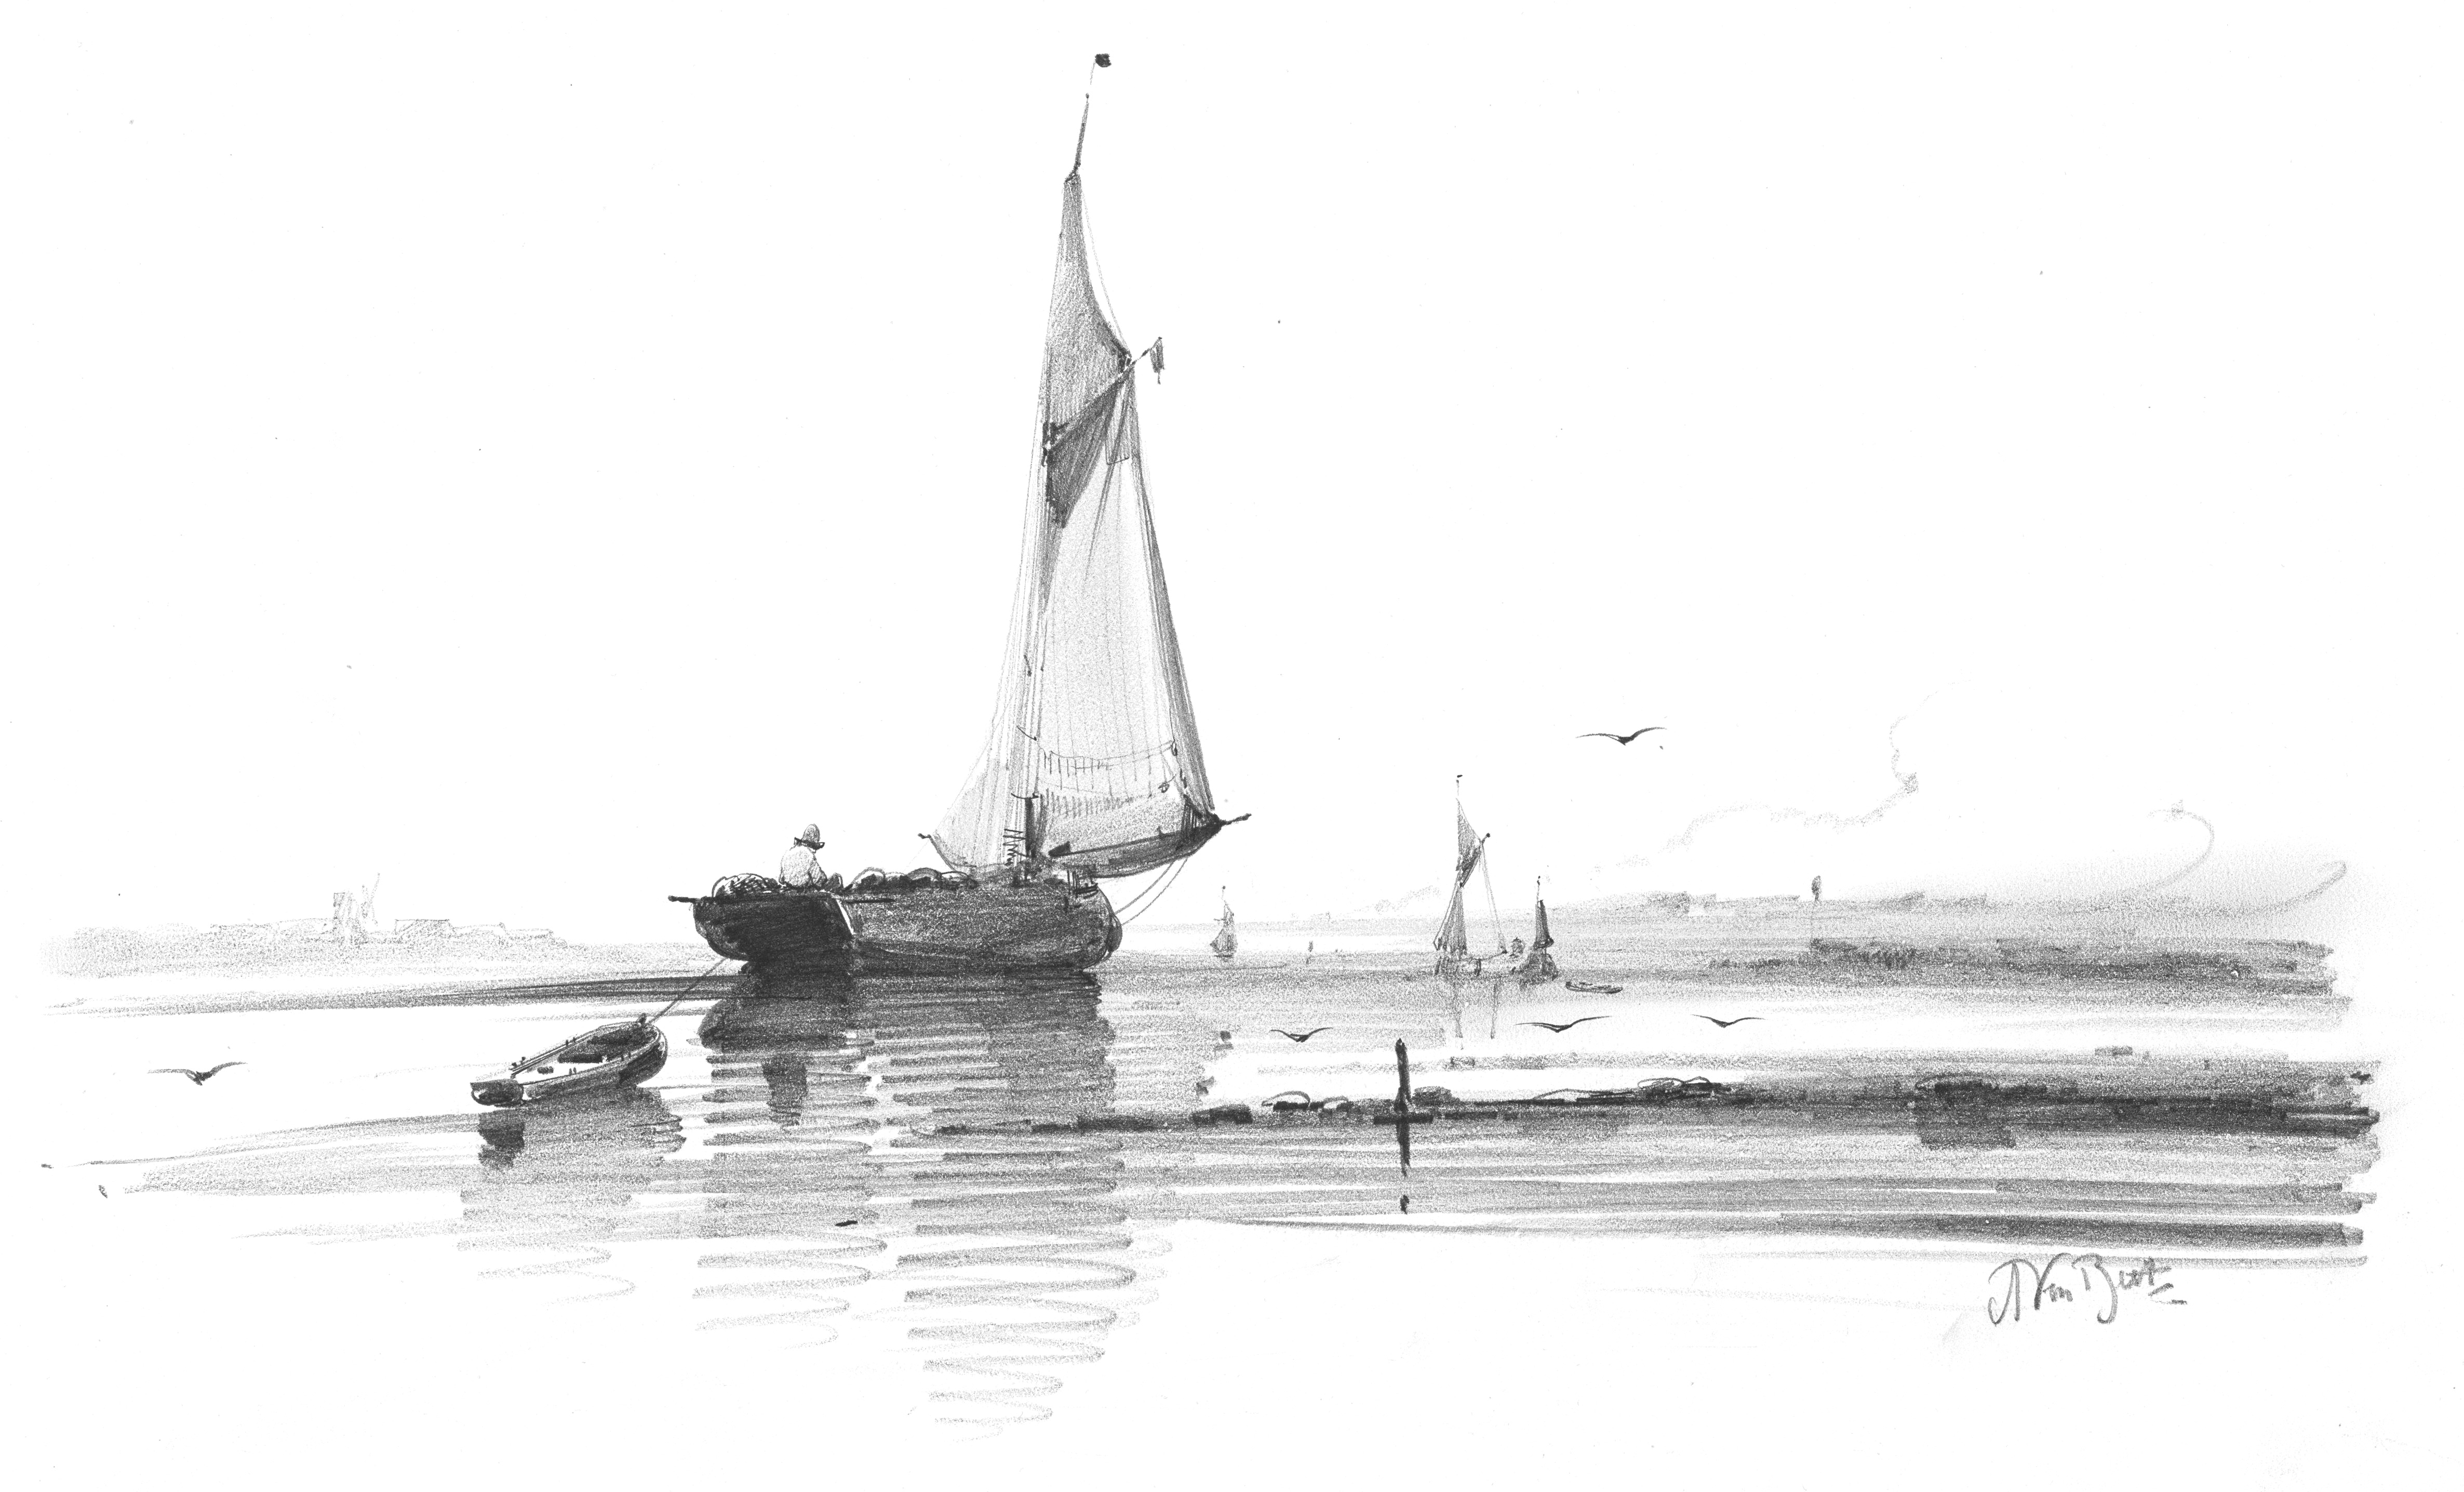
\includegraphics[width=\basicwidth]{sailboat}}
\vfill